\section{Progettazione}\label{progettazione}
\subsection{Base di dati}
OSS possiede una propria base di dati formata da 19 tabelle e 5 viste. Si vogliono mantenere logicamente separati i dati relativi alla PadovaCard.\\

Di seguito venogno riportati lo schema concettuale, lo schema logico e il DDL dell'espansione del database, mentre non viene riportata la struttura del database esistente in quanto non interagirà con le nuove tabelle.\\

Una nota sui nomi delle tabelle è d'obbligo, CackePHP richiede l'utilizzo di una sintassi standard per i nomi delle tabelle, necessaria per effettuare l'accoppiamento model-tabella. Risulta quindi necessario utilizzare nomi inglesi plurali o nomi italiani che terminano per s.
\subsubsection{Modello concettuale}
\begin{figure}[H]
\centering
\includegraphics[width=1\textwidth]{images/concettuale.png}
\caption{Modello concettuale della base di dati}
\end{figure}
L'espansione del database già esistente si compone di 3 tabelle, cards, packets e structures mentre clientis e users sono già presenti.
Le nuove tabelle saranno collegate al database esistente tramite clientis e users utilizzando chiavi esterne.\\ \\
\textbf{Tabelle}
\begin{itemize}
\item \textbf{card:} contiene tutte le informazioni sulle PadovaCard;
\item \textbf{clientis:} contiene l'anagrafica degli utenti che hanno acquistato una PadovaCard o altri articoli che necessitano di anagrafica dal sistema;
\item \textbf{packets:} contiene i dati relativi ai pacchetti associabili alla PadovaCard. Ricordiamo che un pacchetto è un insieme di strutture visitabili;
\item \textbf{structures:} contiene i dati su tutte le strutture convenzionate con PadovaCard;
\item \textbf{users:} contiene i dati relativi agli operatori e al personale delle strutture. In futuro potrebbe contenere anche quelli relativi agli hotel.
\end{itemize}
\textbf{Relazioni}
\begin{itemize}
\item \textbf{appartiene a:} cards è connessa con una relazione uno a molti a clientis perchè ogni utente può avere una sola PadovaCard attiva, ma più di una non attive, ogni Padovacard attiva deve essere connessa ad un cliente, mentre quelle inattive possono non esserlo. Questa distinzione si rende necessaria per quando in futuro gli utenti potranno acquistare via web le PadovaCard. Ci sarà un periodo di tempo tra la creazione della carta e l'inserimento di tutti i nominativi a causa degli ordini di più PadovaCard. Escludendo questo requisito anche le PadovaCard inattive hanno un nominativo associato
\item \textbf{associata a:} cards è connessa con una relazione uno a molti a packets perchè ad ogni PadovaCard è associato un solo pacchetto di strutture, mentre un pacchetto può essere associato a più Padovacard;
\item \textbf{composto da:} packets è collegato con una relazione molti a molti a structures in quanto ogni pacchetto è formato da più strutture ed ogni struttura può essere presente su più pacchetti;
\item \textbf{lavora a:} users è collegato con una relazione uno a molti a strcutures per mantenere i dati relativi al personale delle strutture;
\item \textbf{venduta da:} cards è connessa con una relazione uno a molti ad users in quanto bisogna tener traccia di quale operatore vende una PadovaCard, una Padovacard può essere venduta da un solo operatore e un operatore può vendere più PadovaCard. Una carta può non essere venduta da un operatore, nel caso in cui l'acquisto sia fatto via internet;
\item \textbf{visitato:} cards è connesso con una relazione molti a molti a strutture perchè è necessario tener traccia di quali struttre ha visitato l'utente per impedire che con la stessa PadovaCard venga visitata più volte la stessa struttura.


\end{itemize}


\subsubsection{Modello logico-relazionale}\label{logicorelazionale}

\begin{figure}[H]
\centering
\includegraphics[width=1\textwidth]{images/logico.png}
\caption{Modello logico della base di dati}
\end{figure}
CakePHP prevede che ogni tabella abbia una sola chiave primaria in quanto non supporta chiavi primarie composite, per questo è necessario aggiungere una chiave primaria "di servizio" per CakePHP in tabelle come visite e composizione.\\ \\
\textbf{Note di progettazione}\\ \\
Inizialmente cards conteneva un campo dal nome prenotazionecappella, di tipo datetime, che doveva contenere la data e l'ora della prenotazione alla \cappella. \'E stato deciso di spostare tale campo sulla tabella visits e rinominarlo dataprenotazione. Questo permette di gestire la prenotazione a più strutture nel caso in cui in futuro ci sia tale necessità. \'E altresi vero che la maggior parte dei record avrà Null come valore di dataprenotazione, ma essendo questo di tipo datetime si è stimato uno spreco di memoria nel caso peggiore di meno di 3 Megabyte annui. Il calcolo è il seguente:
Dimensione di datetime $*$ numero stimato di PadovaCard vendute in un anno $*$ numero massimo di strutture per pacchetto = $8byte*20000*15 $. \\

Attualmente per le password vengono usati campi di tipo char(40) ovvero un campo che può contenere fino ad un massimo di 40 caratteri, sufficienti a contenere l'output della funziona hash \glossario{MD5}. Il tirocinante propone di utilizzare un campo char(64) in previsione dell'utilizzo dell'hash \glossario{SHA256}. Tale cambio è motivato nella Sezione \ref{hash}. \\

Nella tabella users è presente un campo username di tipo varchar(255). Nonostante varchar occupi solamente lo spazio per i caratteri effettivamente scritti, quando vengono create le tabelle temporanee durante le query viene allocata la lunghezza massima. Per questo il tirocinante propone di modificare varchar(255) in varchar(25), più che sufficiente per i valori di tale campo. \\

Clientis contiene i campi cap, telefono e note di tipo varchar(25). Il tirocinante propone di modificare il tipo di cap in char(5), telefono in char(11) e note in varchar(255) in quanto tale valore per varchar è il massimo ottenibile con un solo byte di overhead. Codicefiscale che ora ha tipo varchar(16) viene modificato in tipo char(16). \\

La chiave primaria di cards è codicecarta, con tipo char(10). Si è scelto di utilizzare codicecarta e non un id auto increment in quanto è univoca e permette di evitare una join durante la lettura di visits. Questo è ottimale in quanto visits sarà la tabella con più query in lettura, mentre si stima la perdita di efficienza nell'uso di char invece di int inferiore al 20\% nel caso peggiore, considerando la lunghezza del char, il fatto che è indicizzato e che il motore usato è \glossario{INNODB}. \\

Sempre in cards duratacarta è uno samllint. Ad oggi sono previste solo due durate, 48 e 72 ore, per cui un tipo bool sarebbe stato sufficiente ma uno smallint permette di creare più di due tipologie di durata. \\

La tabella packets contiene il campo descrizione di tipo text, ritenuto necessario se si vuole salvare qui la descrizione completa della struttura che apparirà nel sito che l'utente adrà a consultare per ottenere le informazioni sulla PadovaCard. \\

Cards contiene il flag attiva che indica se la carta è stata pagata, e se è quindi valida. Questo flag è settato subito a 1 se il pagamento avviene con contanti o carta di credito, mentre viene posto a 0 in attesa del pagamento con bonifico. \\

Cards contiene un campo nominativo e un campo idcliente. Idcliente viene utilizzato per collegare la PadovaCard all'anagrafica di chi ha effettuato l'ordine, che può essere una persona sia fisica che giuridica. Nominativo contiene il nome del proprietario della PadovaCard e sarà il nome presente nel voucher. Per questo motivo ci potranno essere più PadovaCard attive con lo stesso idcliente mentre il nominativo sarà unico.\\

Per i campi che rappresentano denaro è stato utilizzato il tipo decimal e si è deciso di continuare ad utilizzarlo in quanto non presenta rischi di approssimazione che invece ha il tipo float. \\ \\
\textbf{Tabelle}\\ \\
Nella seguente Sezione verranno descritte nel dettaglio le tabelle che saranno create. Per ogni tabella è fornita una descrizione sul contenuto e un elenco dei suoi campi, comprensivo di tipo e altre note. \\ \\
PK indica che tale campo è \glossario{chiave primaria} della tabella. \\
FK indica che tale campo  è \glossario{chiave esterna} della tabella.\\
\\ \\
CARDS: Contiene tutti i dati relativi alla PadovaCard.
\begin{itemize}
\item codicecarta: varchar(10) \textit{\textless PK\textgreater}
\item idcliente: int \textit{\textless FK\textgreater}
\item pacchetto: int \textit{\textless FK\textgreater}
\item nominativo: varchar(50)
\item codicetlite: varchar(18)
\item codiceopertatore: varchar(25)
\item codicecassa: varchar(25)
\item iniziovalidita: datetime
\item duratacarta: smallint
\item attiva: bool 
\end{itemize}
CLIENTIS: Contiene l'anagrafice degli utenti.
\begin{itemize}
\item id: int \textit{\textless PK\textgreater}
\item ragionesociale: varchar(50)
\item nominativo: varchar(25)
\item indirizzo: varchar(25)
\item localita: varchar(25)
\item nazione: varchar(25)
\item cap: char(5)
\item telefono: char(11)
\item mail: varchar(25)
\item note: varchar(255)
\item privato: float
\item cognome: varchar(50)
\item nome: varchar(50)
\item codicefiscale: char(16)
\end{itemize}
COMPOSITIONS: Tabella creata dalla relazione "composta da", collega le strutture ai pacchetti.
\begin{itemize}
\item id: int \textit{\textless PK\textgreater}
\item idpacchetto: int \textit{\textless FK\textgreater}
\item idstruttura: int \textit{\textless FK\textgreater}
\end{itemize}
PACKETS: Contiene i dati relativi ai pacchetti, composizioni di strutture visitabili.
\begin{itemize}
\item id: int \textit{\textless PK\textgreater}
\item nome: varchar(25)
\item prezzopieno: decimal
\item prezzo: decimal
\item creazione: datetime
\item descrizione: text
\item base: bool
\end{itemize}
STRUCTURES: Contiene i dati relativi alle strutture convenzionate con PadovaCard.
\begin{itemize}
\item id: int \textit{\textless PK\textgreater}
\item nome: varchar(25)
\item prezzopieno: decimal
\item prezzo: decimal
\item orario: datetime
\item giorniapertura: enum('LU','MA','ME','GI','VE','SA','DO')
\item indirizzo: varchar(25)
\end{itemize}
USERS: Contiene i dati riguardanti gli operatori e il personale delle strutture.
\begin{itemize}
\item id: int \textit{\textless PK\textgreater}
\item username: varchar(25)
\item password: char(64)
\item group\_id: int
\item created: datetime
\item modified: datetime
\item email: varchar(25)
\item idstruttura int \textit{\textless FK\textgreater}
\item approvato: bool
\end{itemize}
VISITS: Tabella creata dalla relazione "visitato", tiene traccia di quali strutture sono state visitate da una data PadovaCard, e di eventuali prenotazioni.
\begin{itemize}
\item id INT \textit{\textless PK\textgreater}
\item codicecarta: varchar(10) \textit{\textless FK\textgreater}
\item idstruttura: int \textit{\textless FK\textgreater}
\item visitato: bool
\item datavisita: datetime
\item dataprenotazione: datetime
\end{itemize}
\textbf{Definizione dello schema logico tramite \glossario{DDL} di MySQL}
\lstset{frame=single}
\begin{center}
\begin{lstlisting}
create table clientis (
  id int(11) not null auto_increment,
  ragionesociale varchar(50) default null,
  nominativo varchar(25) default null,
  indirizzo varchar(25) default null,
  localita varchar(25) default null,
  nazione varchar(25) default null,
  cap varchar(25) default null,
  telefono varchar(25) default null,
  mail varchar(50) default null,
  note varchar(25) default null,
  privato float default null,
  cognome varchar(50) default null,
  nome varchar(50) default null,
  codfiscale varchar(16) default null,
  primary key (id)
) ENGINE=InnoDB  DEFAULT CHARSET=utf8 AUTO_INCREMENT=585;

alter table clientis 
	modify column cap char(5),
    modify column telefono char(11),
    modify column note varchar(255);

create table users (
  id int(11) NOT NULL auto_increment,
  username varchar(255) not null,
  password char(40) not null,
  group_id int(11) not null,
  created datetime default null,
  modified datetime default null,
  PRIMARY KEY  (id)
) ENGINE=InnoDB  DEFAULT CHARSET=utf8 AUTO_INCREMENT=51;

alter table users
	modify column password char(64);
    modify column username varchar(25),
    add email varchar(25),
    add approvato bool,
    add idstruttura int,
    add foreign key (idstruttura) references structures (id);

create table packets(
	id int not null auto_increment,
	nome varchar(25) not null,
    prezzopieno decimal default null,
    prezzo decimal default null,
    creazione datetime default null,
	descrizione text default null,
    base bool default 0,
	primary key (id)
)ENGINE=InnoDB DEFAULT CHARSET=utf8; 
	
create table structures(
	id int not null auto_increment,
    nome varchar(25) not null,
    prezzopieno decimal default null,
    prezzo decimal default null,
    orario varchar(25) default null,
    giorniapertura enum('LU','MA','ME','GI','VE','SA','DO') default null,
    indirizzo varchar(25) default null,
	primary key (id)
)ENGINE=InnoDB DEFAULT CHARSET=utf8;

create table compositions(
	id int not null auto_increment,
    idpacchetto int not null,
    idstruttura int not null,
    primary key (id),
    foreign key (idpacchetto) references packets(id),
    foreign key (idstruttura) references structures(id)
)ENGINE=InnoDB DEFAULT CHARSET=utf8;

create table cards(
codicecarta char(10) not null,
idcliente int not null,
pacchetto int not null,
nominativo varchar(50),
codicetlite varchar(18) not null,
codiceoperatore varchar(25),
codicecassa varchar(25),
iniziovalidita datetime,
duratacarta smallint not null,
attiva bool default 0,
foreign key (idcliente) references clientis(id),
foreign key (pacchetto) references packets(id),
primary key (codicecarta)
)ENGINE=InnoDB DEFAULT CHARSET=utf8;
\end{lstlisting}
\end{center}

\subsection{Architettura del sistema}
Di seguito viene riportata l'architettura di OSS ad alto livello, che si rifà all'architettura MVC imposta da CakePHP. 
Successivamente Model e Controller sono mostrati nel dettaglio, indicando le classi che sono state create o modificate. \\

Dopo questa visione d'insieme, nella Sezione \ref{specificacomponenti} per ogni requisito verranno proposti uno o più diagrammi delle attività e di classe e ogni  componente progettata viene collegata ad un requisito e ad una classe generando il tracciamento che si trova nella Sezione \ref{tracciamento}.

\begin{figure}[H]
\centering
\includegraphics[width=1\textwidth]{images/basic_mvc.png}
\caption{Una tipica richiesta MVC in OSS}
\end{figure}

\begin{figure}[H]
\centering
\includegraphics[width=1\textwidth]{images/model.png}
\caption{Pacchetto Model}
\end{figure}

\begin{figure}[H]
\centering
\includegraphics[width=1\textwidth]{images/controller.png}
\caption{Pacchetto Controller}
\end{figure}

\subsection{Funzionamento \tlite}\label{progettazionetlite}
Prima di vedere la specifica tecnica delle singole componenti è bene vedere il funzionamento del software \glossario{\tlite}. \\

Dalla Figura \ref{tlite} si evince il percorso che l'operatore deve compiere per effettuare la prenotazione della visita alla \cappella. Di particolare interesse è mostrare i punti in cui il nuovo processo differisce da quello attuale:
\begin{itemize}
\item Il biglietto venduto sarà a costo zero, questo permette di concludere la prenotazione anche senza conferma di pagamento;
\item Il resoconto dell'ordine va stampato in formato testuale;
\item L'anagrafica del cliente che effettua l'ordina non va inserita tranne che per nome e cognome;
\item \tlite non invia nessuna email all'utente, ma dato che il campo email è da compilare in modo obbligatorio, verrà inserita una email del tipo \textit{prenotazionipadovacard@n-et.it}. Tale casella email ha lo scopo di fare da storico delle prenotazioni.
\end{itemize}
I punti che invece restano invariati sono:
\begin{itemize}
\item Vi è un solo codice \tlite per ogni prenotazione, indipendentemente dal numero di posti riservati;
\item \'E necessario annullare manualmente l'ordine nel caso in cui il cliente non concluda il pagamento su OSS.
\end{itemize}

\tlite permette di stampare il resoconto dell'ordine, per ottenere un file invece di una stampa cartacea è sufficiente creare a livello di sistema operativo (Windows) una finta stampante che stampa su file, ed impostare come output un formato testuale in quanto semplice da analizzare sintatticamente su OSS in un momento successivo.

\begin{figure}[H]
\centering
\includegraphics[width=0.8\textwidth]{images/tlite.png}
\caption{Funzionamento ordine su \tlite \label{tlite}}
\end{figure}

\subsection{Specifica componenti}\label{specificacomponenti}
\subsubsection{Users}
\def\arraystretch{2}
\begin{table}[H]
\centering
\begin{tabular}{|l|l|}
\hline
Model & User \\ \hline
Controller & UsersControllers \\ \hline
View & Users \\ \hline
Requisiti & ROP 14, ROP 15, ROP 16, RFP 18, ROO 19, ROO 20, ROO 21 \\ \hline
\end{tabular}
\caption{Tracciamento componente-requisiti Users}
\end{table}
Questa componente si occupa della gestione degli utenti, dagli amministratori di OSS agli operatori e con l'estensione di OSS si andrà ad aggiungere anche il personale delle strutture.
Dato che il sistema OSS verrà reso accessibile anche all'esterno della rete \net, si è obbligati a rispettare le direttive sulla privacy, per questo sono stati aggiunti il campo email e il campo approvato nella relativa tabella del database  e la possibilità di recuperare autonomamente la password persa. Vi è inoltre l'obbligo di modificare la password ogni sei mesi in quanto il sistema contiene \glossario{dati personali} (Ma non \glossario{dati sensibili}).
Quest'ultima funzionalità è già implementata.

\begin{table}[H]
\centering
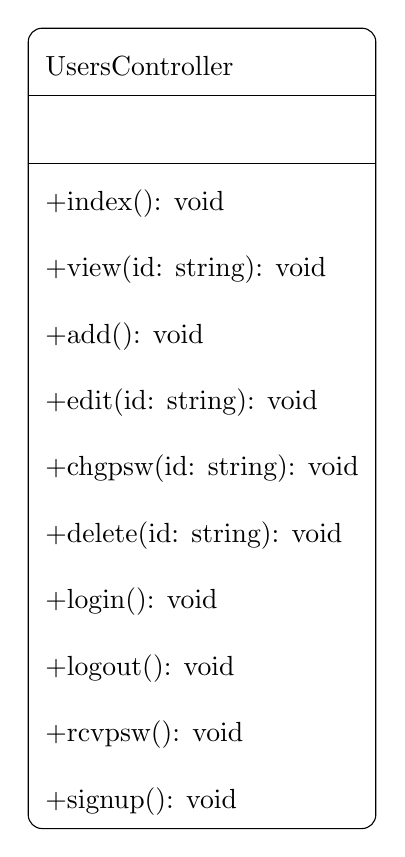
\begin{tikzpicture}
\node (table) [inner sep=0pt] {
\begin{tabular}{l}
  {UsersController} \\
  \hline
  \\
  \hline
  +index(): void \\
  +view(id: string): void  \\
  +add(): void \\
  +edit(id: string): void \\
  +chgpsw(id: string): void \\
  +delete(id: string): void \\
  +login(): void \\
  +logout(): void \\
  +rcvpsw(): void  \\
  +signup(): void  \\
\end{tabular}
};
\draw [rounded corners=.5em] (table.north west) rectangle (table.south east);
\end{tikzpicture}
\caption{Controller:UsersController}
\end{table}



\paragraph{Login}

Il processo di autenticazione esiste già, devono però essere apportate le seguenti modifiche:
\begin{itemize}
\item Nella view va aggiunto un link per il recupero password, che chiamerà il metodo rcvpsw e uno per la registrazione che chiamerà il metodo signup;
\item L'autenticazione dovrà verificare oltre alla corrispondenza username/password anche se tale utente è attivo, controllando se il flag "approvato" è impostato a 1. Questo è possibile farlo aggiungendo l'elemento scope all'array che imposta le opzioni del componente Auth in AppController.php.
\end{itemize}

\label{hash} CakePHP offre la crittazione tramite hash con algoritmo \glossario{MD5}, SHA1, \glossario{SHA256} e blowfish. Attualmete viene utilizzato SHA1. Va tenuto presente però che al momento OSS è un software interno mentre dopo l'espansione verrà reso accessibile anche all'esterno. Per tale motivo il tirocinante suggerisce di passare ad una crittazione più forte come SHA-256, comunque supportata nativamente da CakePHP.

\paragrafo{Diagramma delle attività}

Di seguito è presentato il diagramma delle attività riguardante l'autenticazione a OSS. I soggetti di tali azioni sono operatori e personale.\\

\begin{figure}[H]
\centering
\includegraphics[width=0.8\textwidth]{images/user_login.png}
\caption{Diagramma attività: Login}
\end{figure}

\paragraph{Recupero password}

Il sistema non prevede la possibilità di recupero password, si tratta quindi di una nuova funzionalità. Quando l'utente richiede di recuperare la password:
\begin{itemize}
\item Il sistema genera una passoword casuale di 8 caratteri;
\item Il sistema cripta la passowrd generata con l'algoritmo scelto e salva l'output nel campo password relativo all'utente;
\item Il sistema invia una email con la password all'utente;
\item Nel frattempo l'utente è stato reindirizzato alla pagina di login dove un'avviso gli comunica di controllare la propria casella email;
\item L'utente utilizza la password ricevuta per autenticarsi.
\end{itemize} 

\paragrafo{Diagramma delle attività}
Di seguito è presentato il diagramma delle attività riguardante il recupero password. I soggetti di tali azioni sono operatori e personale.\\


\begin{figure}[H]
\centering
\includegraphics[width=0.6\textwidth]{images/user_rcvpsw.png}
\caption{Diagramma attività: Recupero password}
\end{figure}


\paragraph{Nuovo utente}
Al momento all'interno di OSS sono presente solamente alcuni operatori. Dato che anche il personale delle strutture utilizzerà OSS è necessario che essi possano registrarsi. Non è indicato che sia l'amministratore ad inserirli a sistema in quanto il sistema contiene \glossario{dati sensibili} e dunque la password deve essere conosciuta solo dal proprietario del profilo.

\paragrafo{Diagramma delle attività}
Di seguito è presentato il diagramma delle attività riguardante la creazione di un nuovo utente. I soggetti di tali azioni sono personale e l'amministratore di OSS.\\

\begin{figure}[H]
\centering
\includegraphics[width=0.6\textwidth]{images/user_new_user.png}
\caption{Diagramma attività: Creazione nuovo account}
\end{figure}


\paragraph{Mokup View}
Di seguito un mockup dell'interfaccia utente per la creazione di un nuovo utente.
I mockup di tutti gli altri casi non vengono creati in quanto banali.
\begin{figure}[H]
\centering
\includegraphics[width=0.3\textwidth]{images/mockup_nuovo_utente.png}
\caption{Mockup nuovo utente}
\end{figure}


\subsubsection{Tdocumentos}\label{tdocumentos}
\def\arraystretch{2}
\begin{table}[H]
\centering
\begin{tabular}{|l|l|}
\hline
Model & Tdocumento \\ \hline
Controller & TdocumentosControllers \\ \hline
View & Tdocumentos \\ \hline
Requisiti & ROU 2, ROU 3, ROU 4, ROU 5, RFU 12, ROO 23, ROO 24, ROS 26 \\ \hline
\end{tabular}
\caption{Tracciamento componente-requisiti Tdocumentos}
\end{table}

\begin{table}[H]
\centering
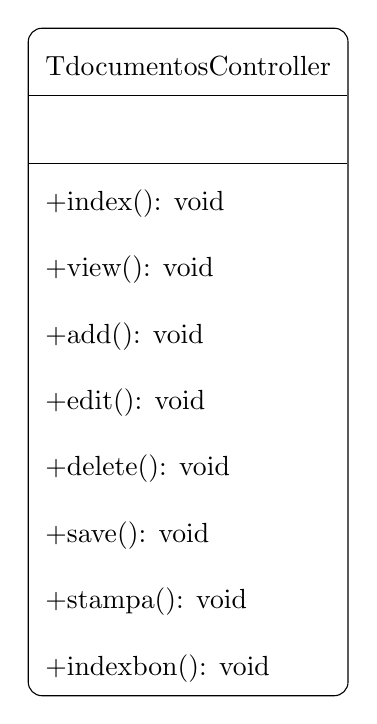
\begin{tikzpicture}
\node (table) [inner sep=0pt] {
\begin{tabular}{l}
  {TdocumentosController} \\
  \hline
  \\
  \hline
  +index(): void \\
  +view(): void \\
  +add(): void \\
  +edit(): void \\
  +delete(): void \\
  +save(): void \\
  +stampa(): void \\
  +indexbon(): void\\
\end{tabular}
};
\draw [rounded corners=.5em] (table.north west) rectangle (table.south east);
\end{tikzpicture}
\caption{Controller:TdocumentosController}
\end{table}


La vendita di un qualsiasi articolo, PadovaCard compresa, al momento inizia da questo controller, con la creazione di un nuovo documento e l'associazione dell'anagrafica di un cliente. \\

Di seguito viene descritto il processo di vendita della PadovaCard attuale:
\begin{itemize}
\item L'operatore seleziona "Nuovo Documento";
\item L'operatore seleziona un anagrafica cliente, o la crea se non esiste;
\item L'operatore sceglie quale PadovaCard vendere;
\item La vendita si conclude con il pagamento.
\end{itemize}
Mentre con il nuovo sistema il processo di vendità diventerà:
\begin{itemize}
\item Da \tlite viene generato un file di testo, come descritto nella Sezione \ref{progettazionetlite};
\item L'operatore seleziona "Nuovo Documento";
\item L'operatore seleziona un anagrafica cliente, o la crea se non esiste;
\item Il file di testo \tlite corrispondente viene caricato;
\item Il sistema ne estrae i seguenti dati:
	\begin{itemize}
        \item Codice operatore;
        \item Codice cassa;
        \item Codice \tlite;
        \item Elenco di data e ora delle varie visite.
	\end{itemize}
\item L'operatore associa ad ogni visita un pacchetto, un nominativo e una data/ora di inizio validità;
\item Il sistema verifica che tale data comprenda al suo interno la visita alla \cappella;
\item L'operatore visualizza il totale e lo comunica al cliente che decide il metodo di pagamento;
\item Con carta di credito la vendita viene conclusa e il sistema invia all'utente inserito su \tlite una mail contenente i voucher e tutti i dati necessari.
\item Con bonifico bancario il sistema invierà una email all'utente specificando i dati per il versamento, quindi a pagamento effettuato\footnote{Gli operatori controllano quotidianamente gli estratti conto del conto corrente} la carta viene spuntata come attiva.
\end{itemize}

\paragrafo{Diagrammi delle attività}

Di seguito è presentato il diagramma delle attività riguardante il processo di vendita di una PadovaCard. 
\begin{figure}[H]
\centering
\includegraphics[width=0.6\textwidth]{images/tdocumentos.png}
\caption{Processo di vendita su OSS}
\end{figure}

\paragraph{Caricamento del file testuale}

Vi sono due possibilità, caricamento manuale o automatico.\\
Con il caricamento manuale è l'operatore che dopo aver cliccato su "Nuova Padova Card" dovrà cliccare su "Carica File" quindi selezionare il file corretto.
Il sistema controllerà che la data di creazione del file non sia troppo precedente alla data di apertura (10 minuti). \\

Con il caricamento automatico l'operatore clicca su "Nuova Padova Card" e quindi su "Carica File" ma è OSS che accede alla cratella in cui si trovano i file, carica tutti i files presenti quindi carica i dati del file di proprietà dell'operatore\footnote{All'interno del file c'è sia il codice operatore che il codice cassa, che sarà confrontato con la login di OSS.}. Una volta caricati i dati su OSS il file viene spostato in una cartella diversa che sarà utilizzata come storico.\\ 

In entrambi i casi è possibile non caricare nessun file, se non vi è nessuna prenotazione da associare, cliccando sul tasto "avanti". \\

Si è deciso di utilizzare il caricamento automatico.

\paragraph{Come vengono estratti i dati dal file} 
Per informazioni sul funzionamento del parser vedere la Sezione \ref{parser}.
Il parser ritornerà le informazioni organizzate in un array di questo tipo:
\begin{lstlisting}
array(
	(int) 0 => array(
		'tlite' => 'TLITE0528719557735',
		'data' => '14/05/2015',
		'ora' => '17:15',
		'numero' => '1'
	),
	(int) 1 => array(
		'tlite' => 'TLITE0528719557740',
		'data' => '14/05/2015',
		'ora' => '17:30',
		'numero' => '2'
	)
)
\end{lstlisting}

\paragraph{Funzionamento del pagamento} 
\paragrafo{Contanti} Il pagamento in contanti prevede un'interfaccia con una semplice calcolatrice per il resto.
\paragrafo{Carta di credito} OSS, cosi come altri gestionali sviluppati da \net utilizza una procedura scritta in PHP che si occupa della creazione di una connessione sicura ai circuiti bancari per il pagamento con carta di credito. Tale procedura è separata dal resto del codice, e non verrà modificata. L'interfaccia prevede il form creato da tale procedura e un link per concludere la vendita.
\paragrafo{Bonifico} Oss rende disponibile un link per inviare al cliente una mail con i dati per il bonifico. Dopo aver inviato la mail è possibile concludere il pagamento. \'E compito degli operatori verificare l'estratto conto, al di fuori di OSS per verificare se il cliente ha versato la somma corretta.

\paragraph{Informazioni in possesso dell'utente al termine del processo} 

L'utente la cui anagrafica è stata inserita a livello di documento è l'unico di cui si conosce l'email, pertanto sarà lui il destinatario della mail contenente le informazioni. Tale mail la cui veste grafica è visible nell'Appendice %TODO 
conterrà le seguenti informazioni:
\begin{itemize}
\item Anagrafica del cliente;
\item Numero di PadovaCard acquistate;
\item Totale pagato;
\item I voucher di ogni PadovaCard, ognuno composto da:
	\begin{itemize}
		\item Codice a barre della PadovaCard;
        \item Codice a barre di \tlite (Se presente);
        \item Strutture visitabili con il pacchetto scelto;
        \item Data e ora della visita alla \cappella (Se presente).
	\end{itemize}
\end{itemize}

\paragraph{Informazioni in possesso del sistema al termine del processo}

Il sistema possiede all'interno della cartella utilizzata come storico i file testuali generati da \tlite. \\

All'interno del database è salvato il log delle operazioni nella tabella log, la transazione nella tabella pagamentos e tutti i dati relativi alla PadovaCard nella tabella cards, consultabile alla Sezione \ref{logicorelazionale}.

\paragraph{Possibili errori} 

Nel caso di caricamento del file manuale potrebbe venir caricato il file errato. \\
Nel caso di caricamento automatico del file, se il file non è stato stampato nella cartella condivisa, potrebbe venir caricato un vecchio file. Questo si risolve sia cancellando i file usati dalla cartella condivisa sia controllando l'ora di creazione del file rispetto all'ora corrente, e avvisando l'operatore se queste differsicono troppo. \\
Nel caso in cui le date di attivazione della PadovaCard fossero discordi con le date delle prenotazioni alla \cappella il sistema avverte l'operatore.
Se i nominativi associati alle PadovaCard sono errati l'utente se ne accorgerà quando riceve l'email, in tal caso dovrà chiamare nuovamente e far modificare i nominativi errati.

\paragraph{Acquisto di altri articoli allo IAT} 

Il requisito ROO24 prevede che venga fatto un unico pagamento agli sportelli IAT nel caso in cui l'utente oltre alle PadovaCard acquisti qualcos'altro. Questo è possibile farlo cliccando su "Nuova Riga", visibile sul menu di sinistra nel mockup \ref{perfezionamentoinfo}. Si verrà reindirizzati all'attuale interfaccia di OSS per la vendita.


\paragraph{Mokup View}
Di seguito un mockup del perfezionamento.

\begin{figure}[H] \label{mockupperfezionamento}
\centering
\includegraphics[width=0.8\textwidth]{images/mockup_perfezionamento_info.png}
\caption{Perfezionamento delle informazioni\label{perfezionamentoinfo}}
\end{figure}


\subsubsection{Cards}
\def\arraystretch{2}
\begin{table}[H]
\centering
\begin{tabular}{|l|l|}
\hline
Model & Card \\ \hline
Controller & CardsControllers \\ \hline
View & Card \\ \hline
Requisiti & ROU 6, ROP 17, ROS 28 \\ \hline
\end{tabular}
\caption{Tracciamento componente-requisiti Cards}
\end{table}

\begin{table}[H]
\centering
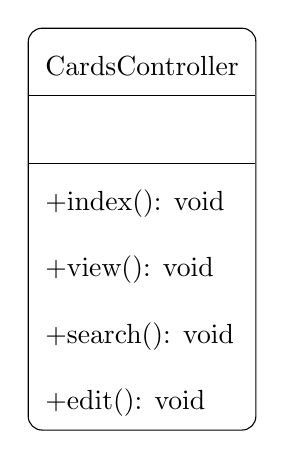
\begin{tikzpicture}
\node (table) [inner sep=0pt] {
\begin{tabular}{l}
  {CardsController} \\
  \hline
  \\
  \hline
  +index(): void \\
  +view(): void \\
  +search(): void \\
  +edit(): void \\
\end{tabular}
};
\draw [rounded corners=.5em] (table.north west) rectangle (table.south east);
\end{tikzpicture}
\caption{Controller:CardsController}
\end{table}

\paragraph{Validazione PadovaCard}
La view collegata ad index corrisponde a quella in figura \ref{validazionecodicebarre}, e permette all'utente di inserire il codice a barre della PadovaCard, manualmente o tramite il lettore.
Il controller index() prende tale valore e recupera le relative informazioni dal database, per poi mostrarle nella view relativa al metodo view. Le informazioni riportate sono:
\begin{itemize}
\item Nome e cognome del possessore della PadovaCard;
\item Data di inizio e fine validità della PadovaCard;
\item Data e ora della visita alla \cappella se si tratta del relativo personale;
\item Validità dell'ingresso, basandosi sul flag "visitato";
\item Se la visita è già stata effettuata, data e ora di tale visita.
\end{itemize}
Dopo aver recuperato le informazioni dal database imposta il flag visitato ad 1, impedendo un ulteriore visita a tale struttura.\\

Si è voluto rendere il più specifici possibile gli errori che la validazione della PadovaCard ritorna, per permettere al personale delle strutture di precisare il motivo per cui l'utente non può visitare la struttura. I possibili errori sono:
\begin{itemize}
\item \textbf{Struttura già visitata}, l'utente cerca di visitare due volte la stessa struttura;
\item \textbf{PadovaCard non attiva}, la PadovaCard è stata disattivata per un qualche motivo che però non è salvato a sistema;
\item \textbf{Struttura non prevista nel pacchetto}, l'utente si reca in una struttura che non fa parte del pacchetto acquistato;
\item \textbf{Data non valida}, l'utente si reca alla struttura in una data al di fuori del range di validità della PadovaCard;
\item \textbf{PadovaCard non valida}, il codice inserito non appartiene a nessuna PadovaCard presente a sistema;
\item \textbf{Leggere l'altro codice}, il codice inserito non è quello della PadovaCard ma quello \tlite, valido solo per la \cappella.
\end{itemize}

\paragrafo{Diagrammi delle attività}
Di seguito è presentato il diagramma delle attività riguardante il processo di verifica di validità di una PadovaCard da parte del personale delle strutture.

\begin{figure}[H]
\centering
\includegraphics[width=0.6\textwidth]{images/validazione_padovacard.png}
\caption{Processo di verifica della validità della PadovaCard}
\end{figure}


\paragrafo{Mokup View}
Di seguito un mockup delle due viste che ha il personale per validare una PadovaCard. Sarà inserito anche un breve tutorial su come leggere le informazioni riportate sulla PadovaCard e su come utilizzare il lettore di codice a barre. Il risultato della lettura sarà mostrato nella stessa pagina, senza bisogno di refresh.
Notare che il focus per la lettura del codice a barre è già sulla casella di input. \\

Questi accorgimenti mirano a semplificare l'interfaccia il più possibile, e a diminuire il numero di click necessari ad operazione, questo perchè molti degli operatori presenti nelle strutture convenzionate sono anziani volontari o membri di categorie protette, che in entrambi i casi non hanno alcuna famigliarità con il computer.
Con gli adattementi descritti un operatore dovrà solamente inserire nome utente e password quindi scansionare con il lettore le PadovaCard, senza toccare mouse o tastiera.
\begin{figure}[H]
\centering
\includegraphics[width=0.5\textwidth]{images/mockup_leggi_barcode.png}
\caption{Schermata per la validazione del codice a barre\label{validazionecodicebarre}}
\end{figure}

\begin{figure}[H]
\centering
\includegraphics[width=0.5\textwidth]{images/mockup_leggi_barcode2.png}
\caption{Risultato validazione}
\end{figure}


\paragraph{Ricerca/Modifica/Stampa PadovaCard}

Le PadovaCard possono essere ricercate utilizzando il loro codice il nominativo del possessore o quello di chi ha effettuato l'ordine. Una volta recuperata una PadovaCard posso modificarla o visualizzare il dettaglio dell'ordine ia cui appartiene e quindi stamparla. \\

Una volta venduta una PadovaCard si possono compiere solo modifiche che non causano una variazione del suo prezzo. Le modifiche possibili sono dunque:
\begin{itemize}
\item Nominativo del possessore, se la ricerca non è stata fatta col nominativo di chi ha effettuato l'ordine;
\item Data/ora di inizio validità;
\item Codice \tlite solo se già presente, non è quindi possibile aggiungerlo o toglierlo.
\end{itemize}
Per quanto riguarda il codice \tlite, se viene modificato sarà l'operatore a dover andare sul software \tlite, annullare la prenotazione relativa al vecchio codice ed effettuarne una nuova per ottenere il nuovo codice. \\

Nel caso in cui la ricerca sia stata fatta con il nominativo di chi ha fatto l'ordine potrò modificare solo la data/ora di inizio validità, ma non per la singola carta, bensì per tutte le carte. Questo per facilitare un cambio di data nel caso di ordini di molte carte (gruppi, scolaresche etc.). \\

Una PadovaCard può essere stampata solamente agli sportelli IAT, in due occasioni:
\begin{enumerate}
\item L'utente è in possesso del voucher, cartaceo o digitale, ma desidera avere la tessera in cartocnino;
\item L'utente ha smarrito la propria PadovaCard e non è in possesso del voucher, si tratta di un caso meno probabile del precedente.
\end{enumerate}
Nel primo caso all'operatore dello IAT basterà utilizzare il lettore dei codice a barre sul codice del voucher per recuperare i dati, quindi avviare la stampa. \\

Il recupero di una PadovaCard smarrita avviene invece tramite nominativo, per cui l'utente dovrà esibire un documento di riconoscimento all'operatore IAT, il quale recupererà i dati tramite nome e cognome, quindi avvierà la stampa. \\	

La stampa è un semplice bottone che avvia in stampa una PadovaCard sull'apposita stampante.

\paragrafo{Mokup View}
Di seguito un mockup della vista che utilizza l'operatore per la ricerca di una PadovaCard.
\begin{figure}[H]
\centering
\includegraphics[width=0.7\textwidth]{images/mockup_stampa_tessera.png}
\caption{Schermata per la ricerca di una PadovaCard\label{stampaPadovaCard}}
\end{figure}

Nell'immagine seguente si vede un mockup della vista per la visualizzazione dei risultati, nella parte superiore può apparire un elenco di PadovaCard tra cui scegliere nel caso in cui la ricerca venga fatta tramite nominativo, e siano presenti più carte appartenenti allo stesso nominativo. Nel caso in cui la ricerca venga fatta tramite intestatario e tale persona ha più ordini salvati nel sistema, si potrà scegliere quale ordine modificare.

\begin{figure}[H]
\centering
\includegraphics[width=0.7\textwidth]{images/mockup_dettagli_ricerca.png}
\caption{Schermata per visualizzare i dettagli di una ricerca}
\end{figure}

\paragrafo{Diagrammi delle attività}
Di seguito è presentato il diagramma delle attività riguardante il processo di modifica della data di validità e del nominativo associati ad una PadovaCard.
\begin{figure}[H]
\centering
\includegraphics[width=1\textwidth]{images/modifica_padovacard.png}
\caption{Processo di modifica dati PadovaCard}
\end{figure}

\subsubsection{Gestione bonifici}
Acquistando tramite call center è possibile effettuare il pagamento via bonifico.
La procedura d'acquisto della PadovaCard rimane uguale a quanto descritto nella Sezione \ref{tdocumentos} e quando si seleziona pagamento tramite bonifico il cliente riceve un email dove vengono specificati conto corrente, causale e importo da versare. Il cliente ha due giorni per effettuare il bonifico e confermare il versamento via email. Gli operatori controlleranno quindi l'estratto conto e in caso positivo concluderanno la vendita e il cliente riceverà i voucher. \\

Oltre all'email con i dati per il pagamento è necessario realizzare un interfaccia che permetta agli operatori di vedere i pagamenti in sospeso e di concluderli. L'index di Tdocumentos mostra già i propri ordini, sia chiusi che pendenti, ma in questo caso ogni operatore ha la necessità di vedere gli ordini di tutti gli operatori in quanto chi effettua l'ordine non è necessariamente colui che lo conclude. Per questo si è deciso di creare una nuova vista dove sono elencati solo i pagamenti via bonifico in attesa di conferma. Per confermare un pagamento si entrerà tramite link alla view dei dettagli dell'ordine. Gli ordini scaduti verranno eliminati.

\paragrafo{Mokup View}
Nell'immagine seguente si vede un mockup della schermata che visualizza i risultati ritornati da una ricerca.

\begin{figure}[H]
\centering
\includegraphics[width=0.7\textwidth]{images/mockup_vista_bonifico.png}
\caption{Schermata per visualizzare i dettagli di una ricerca}
\end{figure}


\subsection{Tracciamento requisiti}\label{tracciamento}

\begin{center}
\def\arraystretch{2}
\begin{longtable}{|p{7cm}|p{3cm}|}
\cellcolor[gray]{0.9} \textbf{Componente} & \cellcolor[gray]{0.9} \textbf{Requisiti} \\ \hline
Users & ROP 14 \newline ROP 15 \newline ROP 16 \newline RFP 18 \newline ROO 19 \newline ROO 20 \newline ROO 21 \\ \hline
Tdocumentos & ROU 2 \newline ROU 3 \newline ROU 4 \newline ROU 5 \newline RFU 12 \newline ROO 23 \newline ROO 24 \newline ROS 26 \\ \hline
Cards & ROU 6 \newline ROP 17 \newline ROS 28 \\ \hline
Cards & ROU 7 \\ \hline
Cards & ROO 25 \newline RFO 31 \\ \hline
\caption{Tracciamento componenti - requisiti}
\end{longtable}

\def\arraystretch{2}
\begin{longtable}{|p{7cm}|p{3cm}|}
\cellcolor[gray]{0.9} \textbf{Requisito} & \cellcolor[gray]{0.9} \textbf{Componenti} \\ \hline
ROU 1 & \\ \hline
ROU 2 & Tdocumentos \\ \hline
ROU 3 & Tdocumentos \\ \hline
ROU 4 & Tdocumentos \\ \hline
ROU 5 & Tdocumentos \\ \hline
ROU 6 & Cards \\ \hline
ROU 7 & Cards \\ \hline
RFU 8 & \\ \hline
RFU 9 & \\ \hline
RFU 10 & \\ \hline
RFU 11 & \\ \hline
RFU 13 & \\ \hline
ROP 14 & User \\ \hline
ROP 15 & User \\ \hline
ROP 16 & User \\ \hline
ROP 17 & Cards \\ \hline
RFP 18 & User \\ \hline
ROO 19 & User \\ \hline
ROO 20 & User \\ \hline
ROO 21 & User \\ \hline
ROO 22 & \tlite \\ \hline
ROO 23 & Tdocumentos \\ \hline
ROO 24 & Tdocumentos \\ \hline
ROO 25 & Cards \\ \hline
ROS 26 & Tdocumentos \\ \hline
ROS 27 & \\ \hline
ROS 28 & Cards \\ \hline
ROS 29 & \\ \hline
RFS 30 & \\ \hline
RFO 31 & Cards \\ \hline
\caption{Tracciamento requisiti - componenti}
\end{longtable}

\end{center} 


% DI TUTTO UN PO'

\subsection{Veste grafica PadovaCard}

La PadovaCard non utilizza bande magnetiche o micro circuiti per essere eco sostenibile, e per lo stesso motivo la scelta del materiale è ricaduta sul cartone. 
Dopo aver provato diversi stampanti si è deciso di adottare il formato \glossario{ISO/IEC 7810:2003 ID-1} che prevede una dimensione di 85,6 mm x 54 mm e gli angoli con un arrotondamento di 3 mm. La stampante scelta vincola la \glossario{grammatura} della carta ad un massimo di 240. \\

Il fronte della PadovaCard manterrà lo stile utilizzato fino ad ora, visibile in Figura \ref{stilepadovacard} che sarà prestampato su ogni PadovaCard.

\begin{figure}[H]
\centering
\includegraphics[width=0.4\textwidth]{images/frontepadovacard.JPG}
\caption{Fronte della PadovaCard \label{stilepadovacard}}
\end{figure}

Il retro verrà invece stampato al momento in quanto contiene le informazioni sulla validità e sul possessore.
Le informazioni sono caricate dal database, quindi utilizzando le librerie descritte nella Sezione \ref{librerie} viene generato un pdf delle esatte dimensioni della PadovaCard.

\begin{figure}[H]
\centering
\includegraphics[width=1\textwidth]{images/retropadovacard.png}
\caption{Retro della PadovaCard}
\end{figure}

\subsection{Parser}\label{parser}
Il parser sarà scritto in PHP e prenderà in input il file testuale stampato da \tlite, sia caricato manualmente sia automaticamente. L'output del parser sarà un array contenente:
\begin{itemize}
	\item Anagrafica del cliente;
    \item Codice operatore;
    \item Codice cassa;
    \item Codice \tlite;
    \item Elenco di data e ora delle varie visite.
\end{itemize}

Il file che viene passato è quello generato dall'operatore attualmente loggato. Ogni riga viene presa singolarmente, e al suo interno vi si cerca una delle parole chiavi che indicano la presenza in tale riga di una delle informazioni ricercate. \\

Quando la riga corretta è individuata, si sostituiscono gli spazi multipli e i caratteri di tabulazione con uno spazio singolo, quindi si esplode la riga in un array, dove ogni elemento è una parola, e si prende l'elemento corrispondente alla posizione dell'informazione cercata all'interno della riga. \\ 

Affinchè il parser funzioni correttamente è necessario che le parole chiavi che vengano ricercate non cambino, e che il numero di parole che precedono l'informazione, per tale riga, non cambi. \\

Nel caso in cui il file non fosse leggibile, o non si trovassero tutte le parole chiave si dirà all'operatore che il file non è stato trovato. \\

Di seguito un esempio del file che il parser prenderà in input.
\lstset{frame=single}
\begin{center}
\begin{lstlisting}[language=TeX]
Ricevuta di Pagamento

                                     Rossi Mario
             Acquistati da    Via Giulio Cesare 01/A 35128 padova (pd) Italia
             
             Codice Transazione                                                      TLITE0528719557700
             
             Evento       Cappella degli Scrovegni e Musei Civici degli Eremitani del 14/05/2015 17:15 
             
             Sala                                                              Cappella degli Scrovegni
             
             Organizzatore                                                             Comune di Padova
             
             Zona                Descrizione posto      Riduzione             N.Bigl.  Prezzo  Prev.
             Ingressi            Ingresso               GRATUITO PADOVACARD     1    0,00   0,00
             
             Totale ricevuta                                                      1          0,00
             
             Gli importi sono comprensivi di iva
             
             Casse e                                                                         PC-01
             operatore                                                                        OperatoreX 
             
             Pagati da
             
             Data emissione                                                            30/01/2015 12:47
             
             Ritiro biglietti
             E' possibile ritirare i biglietti presso la biglietteria del museo a partire dal giorno
             seguente all'acquisto. Il ritiro del biglietto deve avvenire con congruo anticipo: si
             consiglia soprattutto ai gruppi di presentarsi in biglietteria almeno 45 minuti prima
             dell'orario di visita. In caso di acquisto di riduzioni il personale del museo potra'
             richiedere documentazione per verificare l'effettiva validita' dell'acquisto.


\end{lstlisting}
\end{center}
I dati dell'utente si trovano immediatamente sotto la dicitura "Ricevuta di pagamento", il codice \tlite è marcato dalla dicitura "Codice Transazione", data e ora della visita al termine della riga che corrisponde a "Evento" ed infine Cassa e operatore indicano il codice postazione ed il codice dell'operatore  che ha effettuato la vendita.

\subsection{Creazione codice a barre univoco}
Il codice a barre utilizzato è presentato nella sezione \ref{codicebarre}. Di seguito è spiegato come il codice viene generato. \\

Si è scelto di utilizzare l'output della funziona hash SHA-256 più due caratteri, che saranno i secondi del timestamp del log dell'operazione di creazione di una nuova PadovaCard. 
L'input utilizzato per la funzione di hash è dato dal codice \tlite, più un valore di salt, ovvero una sequenza casuale di bit generata da CakePHP.\\

La funzione SHA-256 prende tale input e lo trasforma in una sequenza di 256 bit, siccome nel nostro database abbiamo dichiarato il campo codicecarta di tipo char(10) esso conterrà al più 80bit, per questo motivo tronchiamo i 256 bit di output a 64, cui andranno aggiunti i 16 bit dei restanti due caratteri.\\ 

Grazie all'aggiunta di questi due caratteri si evita il problema di possibili collisioni di input. \\

\'E stato scelto di utilizzare il formato PDF perchè presenta una grafica vettoriale e non raster come ad esempio il formato PNG.
\subsection{Librerie}\label{librerie}
Per velocizzare lo sviluppo ci si è appoggiati a due librerie esterne per la creazione di PDF con all'interno codici a barre.
Tali PDF sono i voucher che il cliente riceve e la PadovaCard che viene stampata.
Entrambe le librerie sono sotto licenza comparabile con la \glossario{MIT} ed è quindi stato possibile modificarle e integrarle nel software.
Le librerie sono le seguenti:\\
\paragrafo{FPDF}
Libreria in PHP che permette di generare file PDF direttamente da PHP, personalizzando il layout e il testo in ogni suo aspetto.\\
\paragrafo{Code-128}
Libreria che appoggiandosi a FPDF permette di generare codici a barre in codifica 128, con la possibilità di scegliere la dimensione e l'orientamento.

\subsection{Codifica codice a barre}
\label{codicebarre}
Esistono due tipologie di codici a barre, lineari e a matrice. \\
Fin da subito si è scelto di utilizzare un codice a barre lineare, scartando quindi codifiche come QrCode e DataMatrix.
Il vincolo per la scelta della codifica lineare da utilizzare è stato imposto dall'azienda fornitrice dei dispositivi di lettura.\\ 

Tra le alternative disponibili due sono state scelte come le più appetibili, la codifica EAN-13 e la codifica 128, su quest'ultima è ricaduta la scelta finale, per due motivi:
\begin{itemize}
\item Permette di rappresentare sia cifre che numeri;
\item \'E disponibile un maggior numero di librerie PHP per la sua creazione.
\end{itemize}

Il codice 128 è un codice a barre lineare ad alta densità, che codifica tutti i caratteri ASCII, dallo 0 al 128 (Da qui il nome).
Ogni singola barra può avere tre diversi significati a seconda di quale dei tre set disponibili è utilizzato, e a seconda del set usato un codice a barre assume un significato diverso.